% !TEX root = macfp_2017_gasphase.tex

\subsection{Different Aspects of Quality Control in CFD: Verification and Validation, Grid Resolution, Physical Modeling} \label{sec:cfd_review}

In this section, we first briefly put the current MaCFP effort in the general context of CFD verification and validation (section~\ref{sec:CVMV}). We then proceed to review the computational challenges associated with simulations of the target experiments selected for the first MaCFP workshop. The challenges include the design of the computational grid (section~\ref{sec:CGD}) and the uncertainties associated with model descriptions of turbulence, combustion and radiation phenomena (section~\ref{sec:PM}).

\subsubsection{Code Verification and Model Validation}
\label{sec:CVMV}

The verification and validation (or V\&V) process is the primary quality control method used to establish the degree of confidence in a computational model for a specific application \cite{ASTM:E1355,Roache:1998,Oberkampf:2006,Oberkampf:2010,McGrattan:2011,FDS_Verification_Guide,FDS_Validation_Guide}. Code \emph{verification} is the process of determining whether the model has been correctly implemented on the computer. In other words, verification ``checks the math".  Model \emph{validation} is the process of determining whether the model correctly represents the physical phenomena of interest. In other words, validation ``checks the physics".  The process of developing a complex fire model is a cycle, as depicted in Fig.~\ref{fig:vv_cycle}, whereby: (1) a mathematical model is proposed; (2) the model is verified; (3) the model is validated; and finally, if modifications to the model are required to achieve more accurate results for the intended application, then the process is repeated.

\begin{figure}
\centering
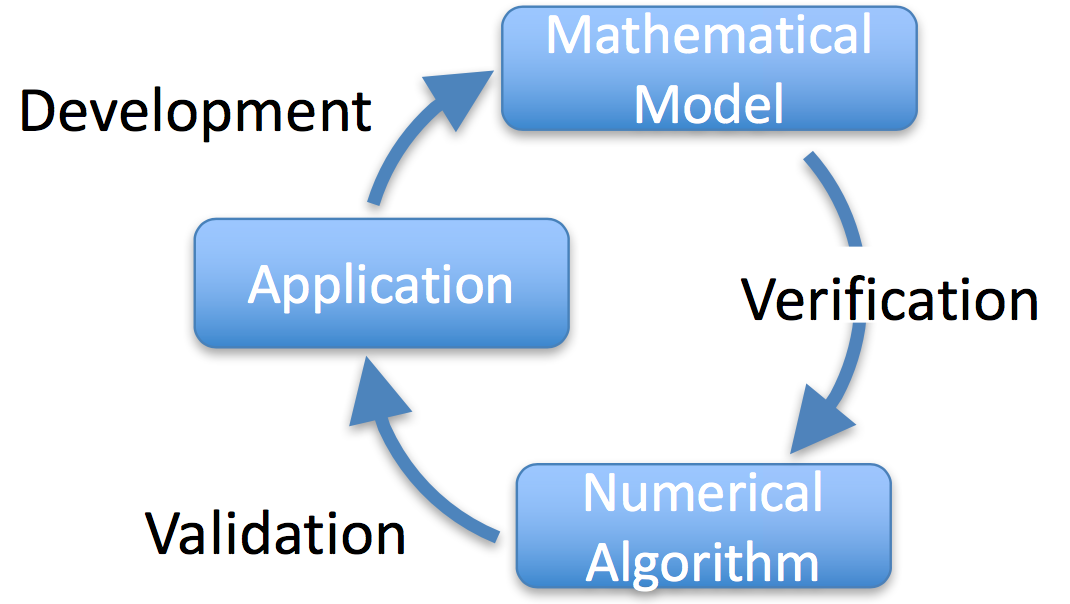
\includegraphics[height=2in]{Figures/vv_cycle.png}
\caption{Schematic representation of the verification and validation process used to evaluate the accuracy of a computational model. Adapted from \cite{Oberkampf:2010}.}
\label{fig:vv_cycle}
\end{figure}

The prevailing technique for verification consists in comparing results of the computational model with analytical solutions (or manufactured solutions \cite{Oberkampf:2010}) obtained for the same system of governing equations. This is usually accomplished through the construction of a library of \emph{unit test} problems. These problems are selected to exercise certain parts of the code (for instance the flow solver --- with or without convection, with or without diffusion, --- the combustion solver, the radiation solver, {\it etc}), considered sequentially and in isolation. The library is constructed with the objective to attain as much ``code coverage'' with unit test problems as possible. Note that MaCFP is not concerned with verification and assumes that the CFD solvers selected for MaCFP activities have been and are continuously verified. MaCFP is focused on validation.

The prevailing technique for validation consists in comparing experimental data with results of the computational model obtained in the same configuration. The target experiments considered in MaCFP correspond to ``open" validation tests in which the modelers have unlimited access to the details of the setup and to the experimental data prior to running the model. In most simulations presented below, the CFD solvers are used in their baseline configuration (presented briefly in section~\ref{sec:PM}), $i.e.$, without resorting to any model modification or calibration, and the simulations can be therefore interpreted as true \emph{validation} tests. In the case of the UMD turbulent line flame experiments, the CFD solvers were used with some advanced features to describe flame extinction that may or may not be part of the baseline configurations. In addition, some of these advanced features were originally tuned against data obtained from the same UMD experiments. In that case, the simulations should be interpreted as \emph{calibration} tests rather than validation tests.

In this first edition of the MaCFP workshop series, no effort was made to impose particular metrics in the comparison between experimental data and simulation results. Comparisons generally take the form of plotting measured and simulated spatial profiles of mean or root-mean-square ({\it rms}) quantities (mean quantities refer to time-averaged quantities and {\it rms} quantities designate the square root of the mean squared deviation of a quantity from its mean). Also no effort was made to require systematic estimates of experimental or numerical uncertainties.

\subsubsection{Computational Grid Design}
\label{sec:CGD}

One of the main challenges found in the application of CFD tools to the simulation of complex flow problems is the design of the computational grid. In large eddy simulations (LES), the design of the computational grid comes from an analysis of the characteristic length scales of the problem and a requirement that large-scale features that (presumably) control the flow dynamics be captured by the grid. The implicit assumption is that small-scale features are dynamically controlled by the resolved scales and can be represented through subgrid-scale (SGS) models. Relevant large-scale features that are considered dynamically-controlling and are therefore grid-resolved in LES of turbulent diffusion flames include: the large flow structures responsible for the production of turbulent kinetic energy (their size is estimated by the integral length scale of the turbulent flow); the large wrinkles on the flame surface responsible for enhanced fuel-air mixing and heat release; and the large soot-containing structures inside and outside the flame zone responsible for flame emission and smoke absorption properties. Small-scale features that are considered dynamically-controlled and remain therefore grid-unresolved in LES include: the small flow structures responsible for the dissipation of turbulent kinetic energy (their size is estimated by the Kolmogorov length scale); the thin reactive layers that make up the micro-structure of a turbulent flame; and the thin elongated soot layers that make up the micro-structure of the flame radiation field.

While the discussion above provides a valuable framework, it is important to emphasize that the separation between large scales that are dynamically-controlling and small scales that are dynamically-controlled is somewhat artificial and is not necessarily obvious. For instance, let us consider the case of a simple pool flame fueled by a liquid chemical supplied through a circular burner of diameter $D$. The pool fire literature suggests that $D$ is the only relevant length scale of the problem: the mean flame vertical height, the mean flame horizontal thickness and the characteristic size of the large turbulent flow structures expected in the flame region are all proportional to $D$ and can be captured in a LES simulation provided that the grid spacing is 10-20 times smaller than $D$.

\begin{figure}
\centering
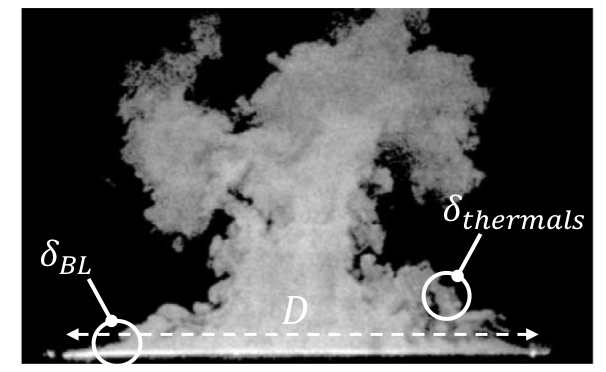
\includegraphics[height=2in]{Figures/He-Plume-Scales.png}
\caption{Illustration of the multi-scale nature of pool fire configurations using a flow visualization of the Sandia helium plume experiment. The configuration features: large-scale structures in the center of the plume with size on the order of the plume diameter $D$; thin boundary layers near the edges of the plume with size $\delta_{BL}$; and small structures created by Rayleigh-Taylor instabilities with size $\delta_{thermals}$. Adapted from \cite{Case1_EXP}.}
\label{fig:He-Plume-Scales}
\end{figure}

However, this is not the whole story. In many cases, the pool flame features a strong buoyancy-driven instability (called the puffing instability) that results in large oscillations in the (horizontal) entrained air flow and the (vertical) combustion products flow. Under strongly unstable conditions, the instantaneous flame takes different shapes during the instability cycle, including the shape of a somewhat unexpected thin (horizontal) boundary layer flame established close to the pool surface and produced by large peak values of the air flow velocity. The presence of the intermittent boundary layer flame is generally over-looked in pool fire studies but circumstantial evidence suggests that it plays an important dynamical role in the instability cycle and consequently needs to be correctly captured by the computational grid. Because its thickness $\delta_{BL}$ is much smaller than the pool diameter $D$, the simulation of the intermittent boundary layer flame brings stringent constraints to the design of the computational grid.

A related topic is the possible development of Rayleigh-Taylor instabilities in regions of the flame with unstable thermal stratification and the associated formation of small plume-like structures, often called ``thermals". When present, these thermals are believed to be responsible for enhanced fuel-air mixing and heat release. Because their characteristic size $\delta_{thermals}$ is much smaller than the pool diameter $D$, the simulation of the thermals brings additional stringent constraints to the design of the computational grid.

Figure~\ref{fig:He-Plume-Scales} presents an illustration of the multi-scale nature of pool fire configurations (albeit in the case of a chemically inert plume) and identifies the three dynamically-controlling length scales: $D$, $\delta_{BL}$ and $\delta_{thermals}$. The dynamic effects occurring at these length scales can be captured in a LES simulation provided that the grid spacing is 10 times smaller than $D$, $\delta_{BL}$ and $\delta_{thermals}$.

We now consider the implications of the previous discussion to the choice of grid resolution in LES simulations of the target experiments selected for the first MaCFP workshop. In the list of six target experiments (Cases 1-5 in section~\ref{sec:intro}), three correspond to pool-like configurations with significant buoyancy-driven instability phenomena ($i.e.$ strong puffing motions and the formation of thermals): the Sandia helium plume; the Sandia methane and hydrogen pool fires; and the UW methanol pool fire. The flow visualization techniques used in these experiments reveal intermittent boundary layers and thermals with length scales on the order of 1~cm, which based on the discussion above, suggests that a millimeter-scale computational grid may be required for accurate simulations. In addition, one target experiment corresponds to a boundary layer flame configuration: the FM Global vertical wall flame. The flow visualization techniques used in this experiment reveal boundary layers and structures with length scales on the order of 1~cm, which again suggests using a millimeter-scale computational grid. Finally, two target experiments correspond to pool-like configurations without reported evidence of a controlling puffing instability: the NIST McCaffrey natural gas flames and the UMD methane and propane turbulent line flames. In the case of the NIST McCaffrey experiments, the only apparent characteristic length scale is the burner size (0.3~m), which suggests using a centimeter-scale computational grid. In the case of the UMD experiments, the only apparent characteristic length scale is the burner width (5~cm), which suggests using a millimeter-scale computational grid.

Note that the numerical submissions to the first MaCFP workshop generally correspond to grid resolutions consistent with the estimates above. In this first edition of the MaCFP workshop series, no effort was made to require systematic grid convergence studies.

\subsubsection{Physical Modeling}
\label{sec:PM}

The numerical submissions to the first MaCFP workshop correspond to one of the following four CFD solvers: FDS, FireFOAM, ISIS and SIERRA/Fuego. All four models are used in LES mode. The solvers differ in details of the formulation of the governing equations, in the construction of the computational grid, in the choice of algorithms used to discretize the governing equations and to provide a numerical solution, and in their ability to perform parallel computing. These differences are believed to be inconsequential in the present tests because the simulations correspond to simple academic configurations. The solvers also differ in the formulation of the physical models used to describe subgrid-scale turbulence, combustion and radiation. These differences are believed to be significant and may be responsible for some or many of the reported discrepancies observed between simulation results, as summarized in the following sections.

In their baseline configuration, the four CFD solvers use:
\begin{itemize}
\item For subgrid-scale turbulence: a classical gradient transport formulation with a SGS turbulent viscosity. A closure expression for the SGS turbulent viscosity is provided by: a modified Deardorff model~\cite{Deardorff:1980} (FDS, see also Ref.~\cite{FDS_Math_Guide}); a model using a (constant-coefficient or dynamic) equation for SGS turbulent kinetic energy~\cite{Fureby:1997} (FireFOAM, SIERRA/Fuego); or the dynamic Smagorinsky model~\cite{Moin:1991} (ISIS).
\item For combustion: a global combustion equation combined with a closure expression for the reaction rates based on either the Eddy Dissipation Model~\cite{Magnussen:1976} (FDS, see also Ref.~\cite{FDS_Math_Guide}, FireFOAM, ISIS) or a steady laminar flamelet model~\cite{SIERRA/Fuego_User_Guide1,SIERRA/Fuego_User_Guide2} (SIERRA/Fuego).
\item For radiation: a treatment based on either a solution of the radiative transfer equation (RTE) combined with a closure expression for the emission term using a prescribed global radiative loss fraction (FDS, see also Ref.~\cite{FDS_Math_Guide}, FireFOAM) or a solution of simplified equations based on the $P$1-approximation (ISIS)  (note that results obtained with SIERRA/Fuego did not use a radiation model).
\end{itemize}

These baseline models have a number of known limitations. First, the SGS turbulence models are models that have been formulated for high-Reynolds-number, momentum-driven flow applications and that may not apply directly to fires which feature moderate-Reynolds-number, buoyancy-driven flow and Rayleigh-Taylor instabilities. Second, the combustion models based on a global combustion equation and the Eddy Dissipation Model are limited to configurations without ignition/extinction phenomena and need to be modified to treat flame extinction in applications to under-ventilated fires or suppressed fires. And third, the radiation models based on a prescribed global radiative loss fraction are limited to configurations in which these fractions have been measured and in which the fire regime does not deviate significantly from the conditions of the measurements.

The identification of these limitations, the quantification of their relative importance, and ultimately their elimination through more advanced models are some of the objectives of the MaCFP effort.





















